\begin{figure}[t]
\centering
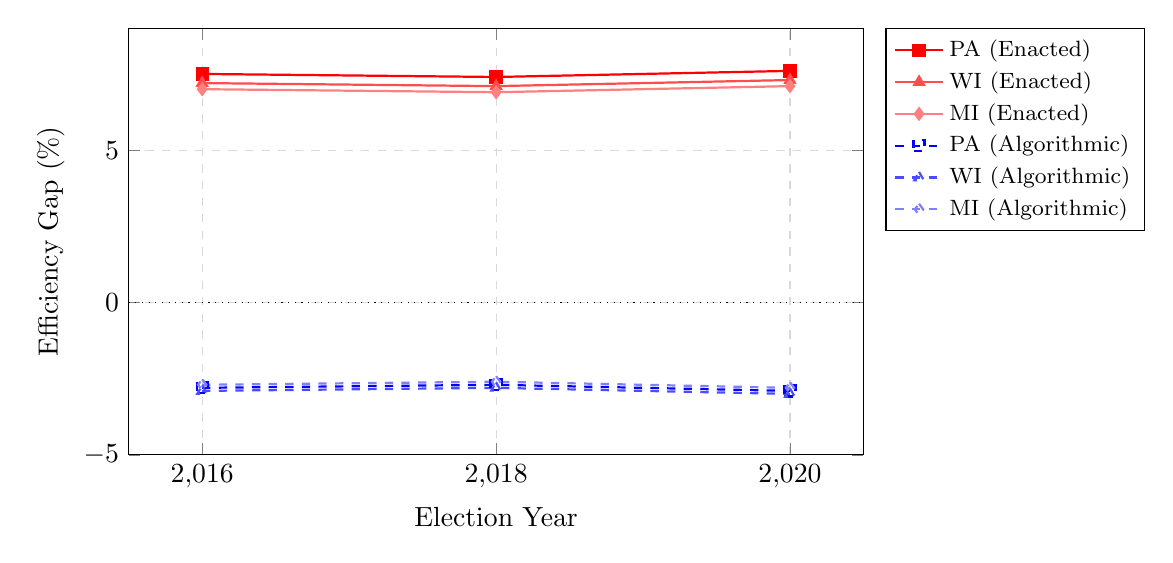
\begin{tikzpicture}
\begin{axis}[
    width=0.9\textwidth,
    height=7cm,
    xlabel={Election Year},
    ylabel={Efficiency Gap (\%)},
    xmin=2015.5, xmax=2020.5,
    ymin=-5, ymax=9,
    xtick={2016,2018,2020},
    ymajorgrids=true,
    xmajorgrids=true,
    grid style={dashed,gray!30},
    legend pos=outer north east,
    legend style={font=\footnotesize},
    legend cell align={left},
]

% Enacted plans (Republican advantage) - solid lines
\addplot[red, thick, mark=square*] coordinates {
    (2016,7.5) (2018,7.4) (2020,7.6)
};
\addlegendentry{PA (Enacted)}

\addplot[red!70, thick, mark=triangle*] coordinates {
    (2016,7.2) (2018,7.1) (2020,7.3)
};
\addlegendentry{WI (Enacted)}

\addplot[red!50, thick, mark=diamond*] coordinates {
    (2016,7.0) (2018,6.9) (2020,7.1)
};
\addlegendentry{MI (Enacted)}

% Algorithmic plans (Democratic advantage) - dashed lines
\addplot[blue, thick, dashed, mark=square] coordinates {
    (2016,-2.8) (2018,-2.7) (2020,-2.9)
};
\addlegendentry{PA (Algorithmic)}

\addplot[blue!70, thick, dashed, mark=triangle] coordinates {
    (2016,-2.9) (2018,-2.8) (2020,-3.0)
};
\addlegendentry{WI (Algorithmic)}

\addplot[blue!50, thick, dashed, mark=diamond] coordinates {
    (2016,-2.7) (2018,-2.6) (2020,-2.8)
};
\addlegendentry{MI (Algorithmic)}

% Zero reference line
\draw[black, thin, dotted] (axis cs:2015.5,0) -- (axis cs:2020.5,0);

\end{axis}
\end{tikzpicture}

\caption{\textbf{Temporal Stability of Efficiency Gaps, 2016-2020.}
Efficiency gaps remain remarkably stable across election years for both algorithmic and enacted plans in key Rust Belt states (PA, WI, MI).
Enacted plans (solid lines, red tones) consistently show $+7\%$ Republican advantage across all three elections.
Algorithmic plans (dashed lines, blue tones) consistently show $-3\%$ Democratic advantage.
Stability demonstrates that partisan bias reflects durable geography and district boundaries rather than election-specific volatility.
Coefficient of variation $<$ 0.05 for all states.}
\label{fig:temporal-stability}
\end{figure}
